\documentclass{beamer} % Use handout to get rid of repeated slides
\usetheme{AnnArbor}
\usecolortheme{default}
\usefonttheme{professionalfonts}
\usepackage{mathpazo}
\usepackage{listings}
\usepackage{xcolor}

% Define colors
\definecolor{myred}{RGB}{163,0,0}
\definecolor{ttcolor}{RGB}{0,0,1}%{RGB}{163,0,0}
\definecolor{mygray}{RGB}{248,249,250} 
\definecolor{mygreen1}{RGB}{0,96,0}
\definecolor{mygreen2}{RGB}{229,239,229}
\definecolor{aristotelgreen}{HTML}{008A44}
\definecolor{aristotelred}{HTML}{9E0101}
\definecolor{aristotelgrey}{HTML}{2E2E2E}
\definecolor{aristoteldarkred}{HTML}{500101}
\definecolor{aristotelorange}{HTML}{FF8C00}

\setbeamertemplate{theorem}[ams style]
\setbeamertemplate{theorems}[numbered]

\usepackage{etoolbox}
\usepackage{amsmath}

\undef{\definition}
\theoremstyle{definition}
\newtheorem{definition}{\translate{Definition}}
\hypersetup{
	colorlinks=true,
	linkcolor=aristotelorange,   % color for normal internal links
	citecolor=aristotelgreen,   % color for citation links
	urlcolor=aristotelgreen      % color for external links
}

\setbeamercolor{palette primary}{bg=aristotelred, fg=white}
\setbeamercolor{palette secondary}{bg=aristoteldarkred, fg=white}
\setbeamercolor{palette tertiary}{bg=black, fg=white} 

\setbeamercolor{title}{fg=white, bg=aristotelred} % Title text color
\setbeamercolor{subtitle}{fg=white, bg=aristotelred} % Subtitle text color
\setbeamercolor{background canvas}{bg=aristotelgrey} % Background for content canvas
\setbeamercolor{normal text}{fg=white} % Normal text color
\setbeamercolor{titlegraphic}{bg=mygray} % Background color for title graphic area
\setbeamercolor{frametitle}{fg=white, bg=aristoteldarkred}

% Change color of numbered circles in the table of contents
\setbeamercolor{section number projected}{bg=white, fg=black}
\setbeamercolor{subsection number projected}{bg=aristotelred, fg=aristotelgrey}
\setbeamercolor{subsection number projected}{bg=aristotelorange, fg=white}


\setbeamercolor{block title}{fg=white,bg=mygreen1}
\setbeamercolor{block body}{fg=black,bg=mygreen2}


\lstdefinestyle{rstyle}%
{language=[LaTeX]TeX,
	basicstyle=\footnotesize\ttfamily,
	backgroundcolor = \color{mygray},
	commentstyle=\slshape\color{green!50!black},
	keywordstyle=\color{blue},
	identifierstyle=\color{blue},
	stringstyle=\color{orange},
	%escapechar=\#,
	rulecolor = \color{mygray}, 
	showstringspaces = false,
	showtabs = false,
	tabsize = 2,
	emphstyle=\color{red},
	frame = single} 


\begin{document}
	
	% Title page information
	\title[Student Performance]{Follow up}
	\subtitle{Predicting First‑Year Statistics Grades
		from Attendance, Honesty, and Quiz Results
		Cohort 2025/29}
	\author[Riste Petrov]{Riste Petrov \\ \href{mailto:riste@uni-sofia.bg}{riste@uni-sofia.bg}}
	\institute[AEEM - FEBA]{AEEM - FEBA - Sofia University St. Kliment Ohridski - coh. 2025/26}
	\titlegraphic{\includegraphics[scale=0.5]{/home/anonymous/Documents/Mega/ЦЕЛ/Master/1Courses/SU ENG White horizontal.pdf}}
	\date{\today}
	
	\begin{frame}
		\titlepage
	\end{frame}
	
	\begin{frame}
		\frametitle{Contents}
		\tableofcontents[]
	\end{frame}
	
	\section{Introduction}
	\begin{frame}
		\frametitle{Introduction}
		As of this February, i started as a Teaching Demonstrator at UGD Shtip. Because of wanting to make the exercise sessions more interactive and to gauge pre-course knowledge on Statistics, unintentionally this experiment was started.\\
		\vspace{1em}		
		Also in order to have an objective way (numeric) of grading the attendance on exercise sessions, homework i started the dataset used in this experiment.\\
		\vspace{1em}
		The grade structure at UGD Shtip is as follows: \\
		\begin{center}
	
		{\small My points for the subject Financial markets and institutions }
		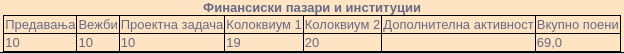
\includegraphics[width=\textwidth]{FPI.png}
		As a Teaching Demonstrator for the cohort i am grading the Exercise Session Points, Course project \& Additional Activity. 
		\end{center}
			 
	\end{frame}
	\subsection{What is collected?}
	
	\begin{frame}
		\frametitle{What Data is collected? 1/5}
		Attendance is based on three attendance measures: 
		\begin{itemize}
		\item Official Attendance list - Faculty demanded
		\item Paper Attendance list - Rewritten every lecture
		\item Digital Quiz Attendance Gathering. 
		
				
		\end{itemize}
		\begin{center}
		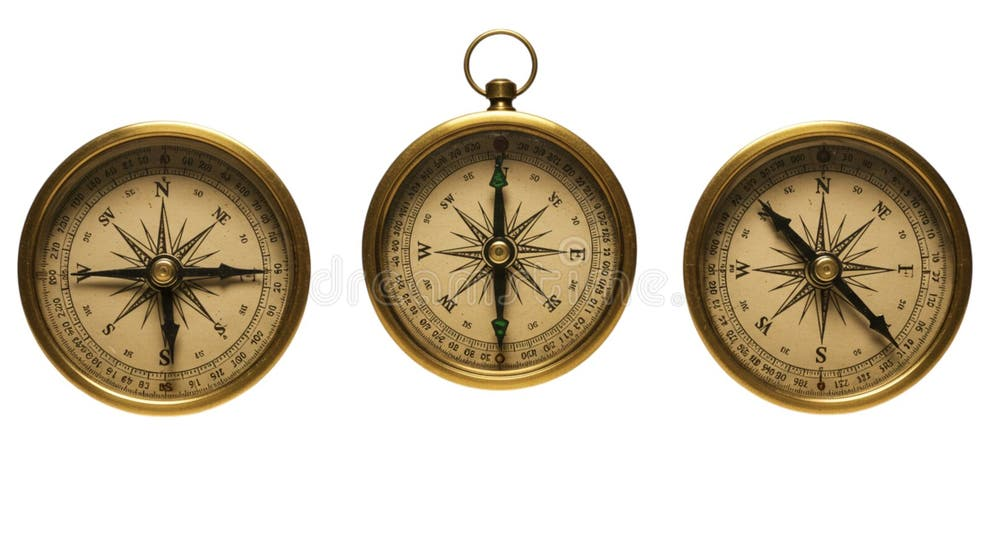
\includegraphics[width=0.5\textwidth]{compases.jpg}
		\end{center}
		20\% of the 10 points for Exercise Session is achieved trough these three compasses - an Average with cutoffs for each mid-term. 
	\end{frame}
	
	\begin{frame}
	\frametitle{What Data is collected? 2/5}
		Homework related data:
		Almost after each lecture with the professor, homework is given which is the other 80\% of the total 10 points for Exercise session:\\
		\vspace{1em}
		\begin{itemize}
			\item Number of homework written
			\item Hand written homework dummy
			\item Late submission of homework dummy 
		\end{itemize}
		
		 
	\end{frame}

	\begin{frame}
		\frametitle{What Data is collected? 3/5}
		Every exercise session, mid session there is a google forms quiz from which apart from the mentioned attendance the following data is extracted:\\
		\vspace{1em}
			\begin{itemize}
				\item Quiz score - measure for student mastery of the material. 
				\item Score of hardness of homework written
				\item Honesty about homework written binary variable - comparing answers with factuals.
			\end{itemize} 
		
		
	\end{frame}

	\begin{frame}
		\frametitle{What Data is collected? 4/5}
		Other data derived from the previously mentioned one:
		\begin{itemize}
			\item Sitting close to .25 percentile - low test score and .75 percentile - high test score influence.
			\item Honesty about the attendance - altering attendance records on the official attendance list. 
			\item Suspected cheating - during the mid-term exam students who turned around or tried forms of workaround, but not doing a misdemeanor to result in a test being taken and having a 3 exam session detention of taking the exam. (approximately 1 year)  
		\end{itemize} 
		
	\end{frame}
	
	\begin{frame}
	\frametitle{What Data is collected? 5/5}
	As mentioned on the first introductory slide, a background and statistical quiz was performed in order to measure the general knowledge of the audience and to adapt the material regarding it. From which the following background data was taken:
	\begin{itemize}
		\item High school graduation type - economic / law specialized, gymnasium, other types of specialized High school
		\item Major enrolled - Five types of majors
		\item Attitude towards Math - 1 - 6 scale
		\item Passed Math - binary 
	\end{itemize} 
	
	\end{frame}
	
	\subsection{How is it collected?}
	\begin{frame}
		\frametitle{How is the data collected? 1/3}
		\centering
		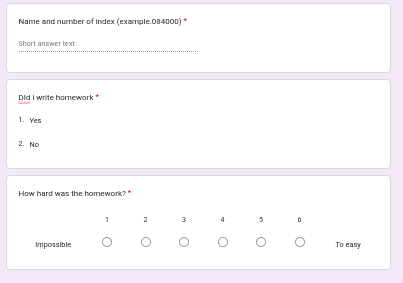
\includegraphics[width=0.8\textwidth]{questioner-every-quiz.png}
	\end{frame}
	
	\begin{frame}
		\frametitle{How is the data collected? 2/3}
		\centering
		\includegraphics[height=0.6\textwidth]{pre-lesson.png}
	\end{frame}
	
	\begin{frame}
		\frametitle{How is the data collected? 3/3}
		\centering
		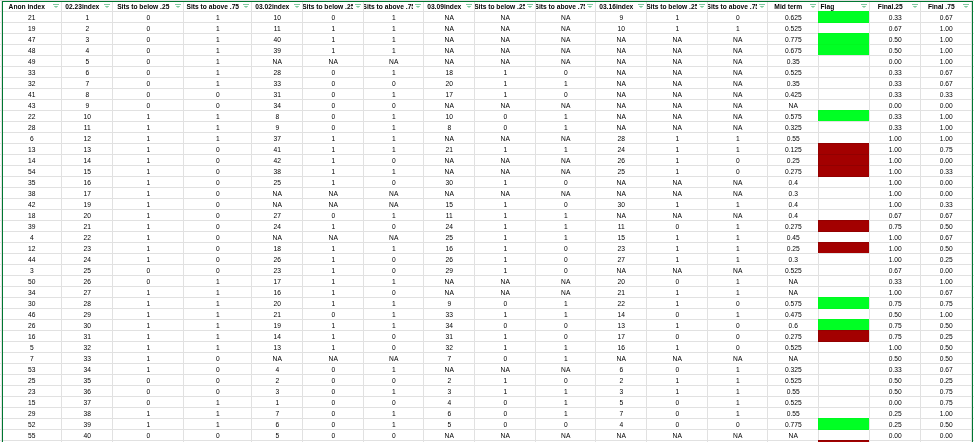
\includegraphics[width=\textwidth]{siting.png}
	\end{frame}
	
	\subsection{Hypotheses}
	\begin{frame}
		\frametitle{Hypotheses}
		\centering
		\begin{itemize}
			\item H0 Attendance, homework completion/timeliness, and academic honesty predict test performance more strongly than attitude toward math.
			\item H1 Seating proximity to lower- or higher-achieving peers affects student performance compared with students near the median.
			\item H2 Lower attendance, late homework submission, digitally completed homework, and low quiz scores are associated with lower final results, and the opposite patterns predict higher results.
		\end{itemize}
	\end{frame}
	
	\subsection{Methods}
	\begin{frame}
		\frametitle{Statistical Methods}
		\centering
		\begin{itemize}
			\item Regressions
			\item ART-2a clustering
		\end{itemize}
	\end{frame}
	
	\section{Examining the hypoteses}
	\subsection{Results}
	\begin{frame}
		\frametitle{Hypothesis 0}
		\centering
		\begin{itemize}
			\item H0 Attendance, homework completion/timeliness, and academic honesty predict test performance more strongly than attitude toward math.
		\end{itemize}
		\vspace{1em}
			\begin{equation*}
				\begin{aligned}
					Y &= \mathrm{averATND} + \mathrm{numHW} + \mathrm{paperHW} + \mathrm{lateHW} \\
					&\quad + \mathrm{additHW} + \mathrm{honLST} + \mathrm{honHW}
					+  \mathrm{atitMATH}
				\end{aligned}
			\end{equation*}
	\end{frame}
	
		\begin{frame}
		\frametitle{Hypothesis 0}
		\centering
		\begin{itemize}
			\item Using OLS with HW errors statistically significant were only the group average Attendance and if the person was suspected of Cheating.
		\end{itemize}
		\vspace{1em}
		\begin{table}[!htbp]
			\centering
			\tiny
			\begin{tabular}{lrrrr}
				\hline
				Variable & Coefficient & Std. Error & t-Statistic & Prob. \\
				\hline
				C & $1.159647$  & $0.183254$  & $6.328075$  & $0.0000$ \\
				group & $-0.151776$ & $0.045661$  & $-3.323938$ & $\textbf{0.0038}$ \\
				averATND & $-0.140418$ & $0.049650$  & $-2.828162$ & $\textbf{0.0111}$ \\
				numHW & $-0.021964$ & $0.064251$  & $-0.341845$ & $0.7364$ \\
				paperHW & $0.143849$  & $0.103936$  & $1.384014$  & $0.1833$ \\
				lateHW & $0.199300$  & $0.132025$  & $1.509566$  & $0.1485$ \\
				CHEAT & $-0.181898$ & $0.052942$  & $-3.435793$ & $\textbf{0.0029}$ \\
				atitMATH & $0.018119$  & $0.014738$  & $1.229392$  & $0.2348$ \\
				\hline
				R-squared & $0.624018$ & Mean dependent var & $0.463462$ &  \\
				Adjusted R-squared & $0.477802$ & S.D. dependent var & $0.163130$ &  \\
				S.E. of regression & $0.117883$ & Akaike info criterion & $-1.190583$ &  \\
				Sum squared resid & $0.250137$ & Schwarz criterion & $-0.803476$ &  \\
				Log likelihood & $23.47758$ & Hannan-Quinn criter. & $-1.079110$ &  \\
				F-statistic & $4.267800$ & Durbin-Watson stat & $2.031867$ &  \\
				Prob(F-statistic) & $0.006096$ & Wald F-statistic & $10.47473$ &  \\
				Prob(Wald F-statistic) & $0.000031$ &  &  &  \\
				\hline
			\end{tabular}
		\end{table}
		
	\end{frame}
	
	\begin{frame}
		\frametitle{Hypothesis 0a}
		\centering 
		\begin{itemize}
			\item The modified OLS model with HW errors statistically significant we still can conclude that at the cut of of 5\% attitude towards Mathematics is statistically insignificant.  
		\end{itemize}
		\vspace{1em}
			\begin{table}[!htbp]
			\centering
			\tiny
			\begin{tabular}{lrrrr}
				\hline
				Variable & Coefficient & Std. Error & t-Statistic & Prob. \\
				\hline
				C & $1.096379$  & $0.171329$  & $6.399253$  & $0.0000$ \\
				group & $-0.173178$ & $0.041489$  & $-4.174036$ & $\textbf{0.0004}$ \\
				averATND & $-0.105257$ & $0.045496$  & $-2.313561$ & $0.0304$ \\
				CHEAT & $-0.156560$ & $0.054328$  & $-2.881771$ & $\textbf{0.0087}$ \\
				atitMATH & $0.025789$  & $0.013545$  & $1.903924$  & $0.0701$ \\
				\hline
				R-squared & $0.564489$ & Mean dependent var & $0.455556$ &  \\
				Adjusted R-squared & $0.485305$ & S.D. dependent var & $0.165153$ &  \\
				S.E. of regression & $0.118485$ & Akaike info criterion & $-1.262489$ &  \\
				Sum squared resid & $0.308850$ & Schwarz criterion & $-1.022519$ &  \\
				Log likelihood & $22.04360$ & Hannan-Quinn criter. & $-1.191133$ &  \\
				F-statistic & $7.128835$ & Durbin-Watson stat & $1.793407$ &  \\
				Prob(F-statistic) & $0.000771$ & Wald F-statistic & $10.33381$ &  \\
				Prob(Wald F-statistic) & $0.000073$ &  &  &  \\
				\hline
			\end{tabular}
		\end{table}
		
	\end{frame}

	\begin{frame}
		\frametitle{Hypothesis 0c}
		\begin{itemize}
			\item From the clustering using ART-2a comparing medians we could notice that except from the outlier in cluster 3, we can conclude that in general across the clusters other factors are more deterministic of the test scores than the reported attitude towards Mathematics.
		\end{itemize}
		\begin{table}
		\tiny
		\begin{tabular}{|c|c|c|c|c|c|c|c|c|c|}
			\hline
			H0 & $\rho^*$ & 0.8 & $\beta$ & 0.85 &  &  &  &  &  \\
			\hline
			Cluster & num. of obs & Y & MATH & ATND & HW & QIZZ & pHW & hLST & hHW \\
			\hline
			MEDIAN & NA & 0.45 & 3 & 3 & 3 & 0.33 & 0.67 & 1 & 1 \\
			\hline
			0 & 2 & 0.2625 & 1 & \underline{\textbf{3.33}} & 0.5 & 0.2949 & 0.1667 & 1.0 & 1 \\
			1 & 3 & 0.425 & 2 & \underline{\textbf{4}} & 3 & \underline{\textbf{0.6431}} & \underline{\textbf{1}} & 1.0 & 1.0 \\
			2 & 4 & 0.4 & 2.5 & \underline{\textbf{3.33}} & 1 & 0.2541 & 0.1667 & 1.0 & 1 \\
			3 & 1 & \underline{\textbf{0.55}} & \underline{\textbf{5}} & 2 & 1 & 0.28 & 0.3333 & 1.0 & 1.0 \\
			4 & 17 & \underline{\textbf{0.525}} & 3 & 3 & 3 & \underline{\textbf{0.3521}} & \underline{\textbf{1}} & 1.0 & 1.0 \\
			\hline
		\end{tabular}
		\end{table}
	\end{frame}
	
	\begin{frame}
		\frametitle{Hypothesis 1}
		\centering
		\begin{itemize}
			\item H1 Seating proximity to lower- or higher-achieving peers affects student performance compared with students near the median.
		\end{itemize}
		\vspace{1em}
		\begin{equation*}
			\begin{aligned}
				Y &= c + proxi.25 + proxi.75
			\end{aligned}
		\end{equation*}
	\end{frame}
	
	
	
	
	\begin{frame}
		\frametitle{Hypothesis 1}
		\centering
		\begin{itemize}
			\item Sitting close to the lower 25\% using the OLS model results in a statistically insignificant results, on the other hand sitting to an student which has a result in the upper 75\% results in an increase of an average increase of 16\%.
		\end{itemize}
	
	\begin{table}[!htbp]
		\centering
		\tiny
		\begin{tabular}{lrrrr}
			\hline
			Variable & Coefficient & Std. Error & t-Statistic & Prob. \\
			\hline
			C & $0.566482$  & $0.104215$  & $5.435677$  & $0.0000$ \\
			GROUP & $-0.109507$ & $0.042365$  & $-2.584854$ & $0.0133$ \\
			PROXI\_25 & $-0.094443$ & $0.074474$  & $-1.268141$ & $\textbf{0.2117}$ \\
			PROXI\_75 & $0.163784$  & $0.066376$  & $2.467520$  & $0.0178$ \\
			\hline
			R-squared & $0.321135$ & Mean dependent var & $0.440761$ &  \\
			Adjusted R-squared & $0.272645$ & S.D. dependent var & $0.163415$ &  \\
			S.E. of regression & $0.139369$ & Akaike info criterion & $-1.020449$ &  \\
			Sum squared resid & $0.815791$ & Schwarz criterion & $-0.861436$ &  \\
			Log likelihood & $27.47032$ & Hannan-Quinn criter. & $-0.960882$ &  \\
			F-statistic & $6.622660$ & Durbin-Watson stat & $1.725964$ &  \\
			Prob(F-statistic) & $0.000915$ & Wald F-statistic & $7.685862$ &  \\
			Prob(Wald F-statistic) & $0.000333$ &  &  &  \\
			\hline
		\end{tabular}
	\end{table}
	\end{frame}
	
	\begin{frame}
		\frametitle{Hypothesis 1a}
		\centering
		\begin{itemize}
			\item Adding the logic dummy of suspected cheating into the OLS model, results in an insignificant effect of it.
		\end{itemize}
	\begin{table}[!htbp]
		\centering
		\tiny
		\begin{tabular}{lrrrr}
			\hline
			Variable & Coefficient & Std. Error & t-Statistic & Prob. \\
			\hline
			C & $0.580085$  & $0.122129$  & $4.749762$  & $0.0000$ \\
			GROUP & $-0.109421$ & $0.042601$  & $-2.568509$ & $0.0140$ \\
			PROXI\_25 & $-0.093502$ & $0.074389$  & $-1.256925$ & $\textbf{0.2159}$ \\
			PROXI\_75 & $0.164181$  & $0.067883$  & $2.418584$  & $0.0201$ \\
			CHEAT & $-0.019142$ & $0.050753$  & $-0.377164$ & $\textbf{0.7080}$ \\
			\hline
			R-squared & $0.323684$ & Mean dependent var & $0.440761$ &  \\
			Adjusted R-squared & $0.257702$ & S.D. dependent var & $0.163415$ &  \\
			S.E. of regression & $0.140793$ & Akaike info criterion & $-0.980732$ &  \\
			Sum squared resid & $0.812728$ & Schwarz criterion & $-0.781967$ &  \\
			Log likelihood & $27.55685$ & Hannan-Quinn criter. & $-0.906274$ &  \\
			F-statistic & $4.905643$ & Durbin-Watson stat & $1.755268$ &  \\
			Prob(F-statistic) & $0.002517$ & Wald F-statistic & $6.565955$ &  \\
			Prob(Wald F-statistic) & $0.000352$ &  &  &  \\
			\hline
		\end{tabular}
	\end{table}
	\end{frame}
	
	\begin{frame}
		\frametitle{Hypothesis 1c-nc}
		\centering
		\begin{itemize}
			\item From the students not suspected of cheating we have the following clusters:
		\end{itemize}
		\begin{table}
			\small
			\begin{tabular}{|c|c|c|c|c|}
				\hline
				H1-noncheater & $\rho^*$ & 0.65 & $\beta$ & 1 \\
				\hline
				Cluster & number of obs & Y & Proxi.25 & Proxi.75 \\
				\hline
				MEDIAN & NA & 0.45 & 0.42 & 0.88 \\
				\hline
				0 & 3 & 0.15 & 0 & 0 \\
				1 & 4 & 0.35 & 1 & 0 \\
				2 & 4 & \underline{\textbf{0.5125}} & 0.415 & 0.875 \\
				3 & 2 &\underline{\textbf{0.5625}} & 0.875 & 0.875 \\
				\hline
			\end{tabular}
		\end{table}
	\end{frame}
	
	\begin{frame}
		\frametitle{Hypothesis 1c-ch}
		\centering
		\begin{itemize}
			\item From the students suspected of cheating we have the following clusters:
		\end{itemize}
		\begin{table}
			\small
			\begin{tabular}{|c|c|c|c|c|}
				\hline
				H1-cheater & $\rho^*$ & 0.65 & $\beta$ & 1 \\
				\hline
				Cluster & number of obs & Y & Proxi.25 & Proxi.75 \\
				\hline
				MEDIAN & NA & 0.47 & 0.67 & 0.5 \\
				\hline
				0 & 14 &\underline{\textbf{0.3125}} & 1 & 0.33 \\
				1 & 4 & \underline{\textbf{0.375}} & 1 & 0.875 \\
				2 & 12 &\underline{\textbf{0.5}} & 0.33 & \underline{\textbf{1}} \\
				3 & 4 & 0.4875 & 0.415 & 0.415 \\
				4 & 2 & \underline{\textbf{0.525}} & 0.585 & 0.125 \\
				\hline
			\end{tabular}
		\end{table}
	\end{frame}
	
	
	
	\begin{frame}
		\frametitle{Hypothesis 2}
		\centering
		\begin{itemize}
			\item H2 Lower attendance, late homework submission, digitally completed homework, and low quiz scores are associated with lower final results, and the opposite patterns predict higher results.
		\end{itemize}
		\vspace{1em}
		\begin{equation*}
			\begin{aligned}
				Y &= \mathrm{averATND} + \mathrm{averQIZZ} + \mathrm{numHW} +   \\
				&\quad + \mathrm{paperHW} + \mathrm{lateHW} + \mathrm{hardHW} 
			\end{aligned}
		\end{equation*}		
	\end{frame}
	
	\begin{frame}
		\frametitle{Hypothesis 2}
		\centering
		\begin{itemize}
			\item Using an OLS model, non  of the purposed variables have an statistically significant effect on the results on the Midterm exam.
		\end{itemize}
		\begin{table}[!htbp]
			\centering
			\tiny
			\begin{tabular}{lrrrr}
				\hline
				Variable & Coefficient & Std. Error & t-Statistic & Prob. \\
				\hline
				C & $0.702047$  & $0.133771$  & $5.248139$  & $0.0000$ \\
				GROUP & $-0.110862$ & $0.067779$  & $-1.635643$ & $0.1120$ \\
				AVERATND & $-0.071208$ & $0.040783$  & $-1.746003$ & $0.0907$ \\
				AVERQIZZ & $0.164981$  & $0.257482$  & $0.640750$  & $0.5264$ \\
				NUMHW & $0.016727$  & $0.053354$  & $0.313518$  & $0.7560$ \\
				PAPERHW & $0.027505$  & $0.115557$  & $0.238021$  & $0.8134$ \\
				LATEHW & $-0.050928$ & $0.132789$  & $-0.383522$ & $0.7040$ \\
				HARDHW & $0.047602$  & $0.202960$  & $0.234540$  & $0.8161$ \\
				\hline
				R-squared & $0.206920$ & Mean dependent var & $0.452564$ &  \\
				Adjusted R-squared & $0.027837$ & S.D. dependent var & $0.165513$ &  \\
				S.E. of regression & $0.163193$ & Akaike info criterion & $-0.607083$ &  \\
				Sum squared resid & $0.825591$ & Schwarz criterion & $-0.265840$ &  \\
				Log likelihood & $19.83813$ & Hannan-Quinn criter. & $-0.484648$ &  \\
				F-statistic & $1.155443$ & Durbin-Watson stat & $0.975067$ &  \\
				Prob(F-statistic) & $0.355879$ & Wald F-statistic & $1.387053$ &  \\
				Prob(Wald F-statistic) & $0.245763$ &  &  &  \\
				\hline
			\end{tabular}
		\end{table}
	\end{frame}
	
	\begin{frame}
		\frametitle{Hypothesis 2c}
		\centering
		\begin{itemize}
			\item The clustering results show us the following clusters:
		\end{itemize}
		\begin{table}
		\tiny
		\begin{tabular}{|c|c|c|c|c|c|c|c|c|}
		\hline
		H2 & $\rho^*$ & 0.65 & $\beta$ & 1 &  &  &  &  \\
		\hline
		Cluster & number of obs & Y & averATND & averQIZZ & numHW & paperHW & lateHW & hardHW \\
		\hline
		MEDIAN & NA & 0.4 & 3 & 0.3 & 2 & 0.33 & 0 & 0.39 \\
		\hline
		0 & 3 & 0.15 & 0 & 0 & 0 & 0 & 0 & 0 \\
		1 & 36 & \underline{\textbf{0.4375}} & 3 & \underline{\textbf{0.3194}} & 3 & \underline{\textbf{0.6667}} & 0 & \underline{\textbf{0.5}} \\
		2 & 13 & 0.275 & 3 & 0.2204 & 1 & 0 & 0 & 0.2778 \\
		3 & 2 & \underline{\textbf{0.5125}} & \underline{\textbf{0.6667}} & 0.1 & 2 & \underline{\textbf{0.5}} & 0 & \underline{\textbf{0.0833}} \\
		\hline
		\end{tabular}
		\end{table}
	\end{frame}
	
	
	\section{Limitations}
	
	\begin{frame}
		\frametitle{Limitations}
		
		  
		\centering
		\begin{itemize}
			\item \textbf{Exam bias}\\
			
			The initial experiment design was to have a separate person (the professor to examine the mid-term exams) to mitigate for potential bias.	But unfortunately this was not applied as the author and the examiner of the exams was me, but as there is little to none space for bias induced error.\\
			This is not a big limitation because of the nature of the subject being solution to exercises, not a matter of explanation of a theory and interpretation of natural language which could induce bias by the examiner. (such as unreadable handwriting, wording, etc.) 
			
			\item \textbf{Small sample size}\\
			
			In fact the sample size is the whole population, the statistical methods mostly have remedies to handle these drawbacks of small sample case of 49 students who took the midterm. Such as reshuffling to get consistent clusters in the case of ART-2a 
		\end{itemize}
	\end{frame}
	
	
	
	
	\section{Q\&A}
	\begin{frame}[fragile]
		\frametitle{Ending remarks}
		\begin{center}
			I am delighted for your attention.\\
			\vspace{1em}
			Q \& A?
		\end{center}
	\end{frame}
	
	
\end{document}